
\newcommand{\dr} {\ensuremath{\Delta R({\rm lepton},{\rm jet})}}
\newcommand{\pmasym}[2]{^{+#1}_{-#2}}
\newcommand{\sigmattbar}{\ensuremath{\sigma_{\ttbar}}}
\newcommand{\sigmaz}{\ensuremath{\sigma_{\Zboson}}}
\newcommand{\lumitot}{\mbox{0.70~fb$^{-1}$}}
\newcommand{\lumitotpm}{\mbox{0.70$\pm$0.03~fb$^{-1}$}}

%\newcommand{\sigmattbar}{\ensuremath{\sigma_{\ttbar}}}
%\newcommand{\sigmaz}{\ensuremath{\sigma_{\Zboson}}}
%\newcommand{\lumitot}{\mbox{0.70~fb$^{-1}$}}
%\newcommand{\lumitotpm}{\mbox{0.70$\pm$0.03~fb$^{-1}$}}
%cut & count numbers:
\newcommand{\xsectot}{171}
\newcommand{\xsecstat}{\pm 6}
\newcommand{\xsecsyst}{\pmasym{16}{14}}
\newcommand{\xseclumi}{\pm 8}

%cut & count w btagging numbers? or the simultaneous fit?
\newcommand{\xsecbtot}{177}
\newcommand{\xsecbstat}{\pm 6}
\newcommand{\xsecbsyst}{\pmasym {17}{14}}
\newcommand{\xsecblumi}{\pmasym {8}{7}}


\newcommand{\AKT}{anti-k$_{t}$}
\def\lum{{\ensuremath{\cal L}}}
\def \intlum {\int {\cal L} dt}
\def\MCatNLO{{\sc MC@NLO}}
\def\FigMerit{F_M}
\def\JetProb{{\sc JetProb}}
\def\SVZero{{\sc SV0}}
\def\Nn{N_n}  %  ntags in an event
\def\Zg{\Zboson/\gamma^{*}}
\def\GEANT{{\sc GEANT4}}

\section{Dilepton}

%\subsection{Introduction}

While the branching ratio into the dilepton decay channel for top-quark pair production events
isn't as high as the lepton+jets channel, the presence of two high pt-leptons in the final state
makes this a powerful channel for precision measurements of top quark processes.

We here describe a measurement of the top-quark pair-production cross-section using the
dilepton final state, which is characterized by two high-pt, opposite-sign leptons,
significant missing energy due to the presence of neutrinos from the decay of W-bosons,
and two $b$-jets from the decay of the top quarks.


%% Top-quark production in dilepton final states has been studied using
%% proton-antiproton collisions at
%% $\sqrt{s}=1.96~\TeV$~\cite{Aaltonen:2010bs,Abazov:2009ae} and
%% Large Hadron Collider (LHC)
%% measurements of the production cross section in proton-proton
%% collisions at $\sqrt{s}=7~\TeV$ in the same final state have recently been
%% reported~\cite{Chatrchyan:2011nb,ATL-CONF-2011-034}.
%% A measurement is presented of the \ttbar\ production cross section
%% using the dilepton channel, characterized by two opposite-sign
%% leptons, unbalanced transverse momentum indicating the presence of
%% neutrinos from the $W$-boson decays, and two $b$-quark jets. This
%% result uses twenty times more data than the previous ATLAS measurement in the same final state,
%% reported in Ref.~\cite{ATL-CONF-2011-034}.

The high efficiency of lepton selection and the relatively small contribution of backgrounds
to the dilepton final state %combined with a requirement on a $b$-jet that further reduces background 
gives this channel a strong signal-to-background ratio.
The dilepton decay topology is divided into three sub-channels based on the flavor of the
final-state leptons.
The $ee$ channel contains two high-pt, isolated leptons identified using 
the inner detector and the electromagnetic calorimeter, the $\mu\mu$ channel contains two
high-pt, isolated muons which have been identified using the inner detector as well as the muon
spectrometer, and the $e \mu$ final state contains an electron and a muon.
These channels are mutually exclusive to facilitate their statistical combination.


%% The \ttbar~dilepton final states can be selected with a good
%% signal-to-background ratio using simple kinematic requirements.  With
%% the additional requirement of the
%% presence of a jet consistent with a $b$~quark
%% (`$b$-tag'), the signal-to-background ratio can be further improved.
%% Cross-section measurements with and without the $b$-tag requirement
%% are reported here.
%%  Leptons are either well-identified electron or
%% muon candidates that are selected using the full detector or, to
%% reduce losses from lepton identification inefficiencies, isolated
%% tracks.  The well-identified electrons or muons are called
%% `identified leptons', and the isolated tracks are referred to as
%% `track leptons'. The term `lepton' is used to refer to identified
%% leptons and track leptons collectively. Events with one identified
%% lepton and one track lepton are called `lepton+track' events.
%%   Each dilepton channel is
%% exclusive, i.e. has no overlap with the other channels. Channels
%% with tau leptons are not explicitly reconstructed, but reconstructed
%% leptons can arise from leptonic tau decays and a track lepton can
%% arise from hadronic tau decay modes as well.  The analysis with the
%% $b$-tag requirement uses only identified leptons.

The analysis uses collision data with a center-of-mass energy of
$\sqrt{s}$ = 7~\TeV\ from 2011, with an integrated luminosity of \lumitotpm~\cite{lumiPub, lumi}.
The main backgrounds considered in this analysis come from
$\Z$+jets events, events with a single top quark,
diboson events, and events with misidentified leptons originating from hadronic activity.
Background contributions from
$\Zg \rightarrow ee$+jets, $\Zg \rightarrow\mu\mu$+jets and events with
misidentified leptons are estimated using data-driven techniques, and all
other background estimations are obtained using Monte Carlo simulation.


%% The measured cross section takes into account the $\ttbar$\ signal
%% acceptance and the expected background contributions from
%% $\Zg$+jets, single top quarks, $WW$, $WZ$, and $ZZ$ events, and
%% events with misidentified leptons (primarily $W+$jets events).
%% Background contributions from
%% $\Zg\rightarrow ee$+jets, $\Zg\rightarrow\mu\mu$+jets and events with
%% misidentified leptons are evaluated
%% directly from the data. All other background contributions are
%% evaluated using Monte Carlo (MC) simulation samples.


\subsection{Monte Carlo Simulation}
\label{s:mc}


Monte Carlo simulation is used to estimate the production rate and kinematic distributions of the $\ttbar$ signal as well as several important background, 
and in addition it is used to evaluate the size of many important sources of systematic uncertianty.
All Monte Carlo samples used in this analysis were generated using \GEANT~\cite{geant4}\
to simulate the ATLAS detector.


%% Monte Carlo simulation samples are used to calculate the $\ttbar$\
%% acceptance and to evaluate the background contributions from single
%% top quarks, $WW$, $WZ$, and $ZZ$ events, and $\Zg
%% \rightarrow\tau\tau$+jets.
%% All MC samples are processed with the
%% \GEANT~\cite{geant4}\ simulation of the ATLAS detector~\cite{atlsim}\
%% and events are passed through the same analysis chain as the data.

Events containing top quarks, including the $\ttbar$ signal and the single-top background,
were generated using \MCatNLO\ generator~\cite{mcatnlo1,Frixione:2003ei,Frixione:2005vw}\
with the CTEQ6.6~\cite{cteq66}\ parton distribution function (PDF)
set and a top-quark mass of 172.5~\GeV.
However, the reference for the overall $\ttbar$ cross-section was calculated using
{\sc Hathor}\cite{Aliev:2010}, which employs an NNLO perturbative QCD calculation.


%% The generation of \ttbar{} and single top-quark events uses the
%% \MCatNLO\ generator~\cite{mcatnlo1,Frixione:2003ei,Frixione:2005vw}\
%% with the CTEQ6.6~\cite{cteq66}\ parton distribution function (PDF)
%% set and a top-quark mass of 172.5~\GeV. Expected $\ttbar$\ yields
%% are calculated with a cross section normalized to the prediction of
%% {\sc Hathor}\cite{Aliev:2010}, which employs an NNLO perturbative QCD calculation.
%% Single top-quark production with \MCatNLO\ includes the $s$, $t$ and
%% $Wt$ channels and the diagram-removal scheme~\cite{diagrem}\  is
%% used to reduce overlap with the $\ttbar$\ final state.

Drell-Yan events are simulated using the {\sc Alpgen} generator using
CTEQ6L1 \cite{cteq6l}\ to model the parton distribution function (pdf),
and the overall cross-section is scaled to the NNLO prediction, which
requires a scale factor (k-factor) of 1.25.
Diboson events are also modeled using the {\sc Alpgen}\ generator
and the overall cross-sections of the three categories of diboson events
were each individually scaled to match their predictions from NLO QCD,
which were calculated using the MCFM program~\cite{Campbell:1999ah}.

%% Drell-Yan events ($\Zg$+jets) are modeled with the {\sc Alpgen}
%% generator, using the MLM matching scheme~\cite{alpgen}\ and the
%% CTEQ6L1 \cite{cteq6l}\ PDF set. The $\Zg$+jets samples, including
%% both light and heavy flavor jets, are normalized to NNLO with a
%% $K$-factor of 1.25. %~\cite{CSCbook}.
%% In the $\Zg\rightarrow ee$ and $\mu\mu$ decay channels, the
%% background from $\Zg$+jets is evaluated using a data-driven
%% technique that normalizes the MC expectation to the data observation
%% near the $Z$ pole. Background contributions from the $W$+jets final
%% states come primarily from events where the $W$\ boson decays
%% leptonically and the second lepton candidate is a misidentified jet
%% or a heavy-flavor decay. Backgrounds from $W$+jets %and multijet
%% events are evaluated from the data.

All simulated event uses the {\sc Herwig} to model the parton shower ~\cite{herwig1,Corcella:2002jc}
as well as {\sc Jimmy} to simulate the effect of the underlying event model~\cite{jimmy}.
In addition, all events include additional background interactions, generated using Pythia,
to simulate the effect of in-time pile-up at the LHC.
Individual simulation events have been re-weighed so the overall distribution of
additional events due to pile-up matches the distribution measured in data.

%% All MC simulated events are hadronized using the {\sc Herwig}\ shower model~\cite{herwig1,Corcella:2002jc}\ supplemented by the
%% {\sc Jimmy}\ underlying event model~\cite{jimmy}.
%% Both hadronization programs are tuned to ATLAS data using the ATLAS MC10 tune~\cite{ATLAS:1303025}.
%% Diboson events are modeled using the {\sc Alpgen}\ generator normalized with
%% $K$-factors of 1.26 ($WW$), 1.28 ($WZ$) and 1.30 ($ZZ$) to match the total cross section from NLO QCD
%% predictions using calculations with the MCFM program~\cite{Campbell:1999ah}.

%% All Monte Carlo samples are generated taking into account that
%% multiple $pp$ interactions can occur in the same LHC bunch crossing
%% within a given event (`pile-up').  The MC events are re-weighted so
%% that the distribution of interactions per crossing in the MC matches
%% that observed in the data.  The average number of interactions per
%% crossing is 5.6 in this data set.


\subsection{Object selection}
\label{s:object}

The criteria for identifiying physical objects is consistent across the three dilepton sub-channels.
%Both electrons and muons are triggered using a single-lepton trigger

Electrons are identified as clusters in the electromagnetic calorimeter
that are matched to charged tracks in the inner-detector.
Electrons used in this analysis must meet the ``tight'' identification criteria,
which places strict requirements on the quality of the inner detector track and the
shape of the shower in the calorimeter.
Electrons are required to have $\pt>25\GeV$, are required to be within the range of the
optimal ATLAS inner detector, namely having $|\eta_{\text cl}|<2.47$ excluding the
transition region defined by $1.37<|\eta_{\text cl}|<1.52$.
Further, electrons are required to be isolated the electromagnetic calorimeter
by requiring that the transverse energy not associated with the electron within 
a radius defined by $\Delta R\equiv\sqrt{\Delta\eta^2 + \Delta\phi^2}$ must be less than $3.5\GeV$.

%% Lepton isolation requirements reduce backgrounds from misidentified
%% jets and suppress the selection of leptons from heavy-flavor decays.
%% For electron candidates, the transverse energy ($\ET$) deposited in
%% the calorimeter not associated to the electron is summed in a cone
%%  of radius $\Delta R = 0.2$, where
%% electron and is required to be less than $3.5\GeV$.


%% Leptons are required to be isolated and have high transverse
%% momentum, $\pt$, consistent with originating from $W$-boson
%% decay, with $\pt$ thresholds chosen to ensure events are triggered
%% with high efficiency.

%% Electron candidates are reconstructed from energy deposits
%% (clusters) in the EM calorimeter, which are then associated to
%% reconstructed tracks of charged particles in the inner detector.
%% Stringent quality requirements on the conditions of the EM
%% calorimeter at the time of data taking are applied to ensure a well measured reconstructed
%% energy. A `tight' selection~\cite{ElectronPerformance} using calorimeter,
%% tracking and combined variables, is employed to provide good
%% separation between the signal electrons and background.  Electron
%% candidates are additionally required to have $\pt>25\GeV$ and
%% $|\eta_{\text cl}|<2.47$, excluding electrons from the transition
%% region between the barrel and endcap calorimeters defined by
%% $1.37<|\eta_{\text cl}|<1.52$. The variable $\eta_{\text cl}$\ is
%% the pseudorapidity of the energy cluster associated with
%% the candidate.

Muons are required to contain a spectrometer track that matches a track in the inner detector.
They must have $\pt>20\GeV$ and $|\eta|<2.5$.
They are required to be energetically isolated both in the muon spectrometer and in the
inner detector.
The sum of the momenta of tracks having within $\Delta R = 0.3$\ and having $\pt>1$~GeV
must be no more than 4~GeV and the sum of transverse momentum within
a cone of $\Delta R = 0.3$\ must also be less than 4~GeV.
In addition, muons must be separated by at least $\Delta R > 0.4$\ from
selected jets wtih $\pt>20$~GeV, and potential muon pairs coming from
cosmic rays are eliminated by rejecting back-to-back muons with $|d_0|~>~0.5~$mm.

%% Muon candidate reconstruction is begun by searching for track
%% segments in
%%  layers of the muon chambers.
%% These segments are  combined starting from the
%% outermost layer, fitted to account for material effects, and matched
%% with tracks found in the inner detector.
%% The candidates are refitted using the complete track information from
%% both detector systems%~\cite{CSCbook}
%% , and required to satisfy $\pt>20\GeV$ and
%% $|\eta|<2.5$.

%For muon candidates, both the
%corresponding calorimeter isolation energy and the analogous track
%isolation, the sum of the track transverse momenta for tracks with
%$\pt>1$~GeV and in a cone $\Delta R = 0.3$\ centered on the lepton
%candidate, must be less than 4~GeV.

%% Additionally, muon candidates
%% must have a distance $\Delta R > 0.4$\ from any jet with
%% $\pt>20$~GeV, further suppressing muon candidates from heavy flavor
%% decays.
%% Muon candidates arising from cosmic rays are rejected by removing
%% candidate pairs that are back-to-back in the $r-\phi$ plane and
%% with transverse impact parameters relative to the beam axis
%% $|d_0|~>~0.5~$mm.

% Ignore Track Leptons

%% Track-lepton (TL) candidates are defined by an ID track with $\pt >
%% 25\GeV$ and a series of quality cuts optimized for high efficiency
%% and a low rate of misidentification. The track must have at least
%% six  SCT hits  and at least one hit in the innermost pixel layer. It
%% also must have $|d_0| < 0.2$~mm and the uncertainty on the momentum
%% measurement must be less than 20\%. The track has to be isolated
%% from other nearby tracks, following the track isolation defined above, in this case using
%%  tracks with $\pt>0.5\GeV$.  The summed momentum cut is set to 2~GeV.

Jets are reconstructed from energy clusters in the calorimeter using the {\it \AKT} algorithm~\cite{antikt}
with a radius parameter $R = 0.4$.
Jets are calibrated to the hadronic energy scale using $\eta$ and $\phi$ dependent corrections.
Because both jets and electrons are seeded by energy clusters in the calorimeter,
reconstructed jets within $\Delta R=0.2$\ of a selected electron are removed to
prevent double counting of physical objects.
Finally, jets are required to have $\pt>25$~GeV and $|\eta|<2.5$.

%% %of adjacent calorimeter cells.
%% These jets are then calibrated to
%% %by first
%% %correcting the jet energy using the scale established for
%% %electromagnetic objects and then performing a further correction to
%% the hadronic energy scale using $\pt$\ and $\eta$\ dependent
%% correction factors~\cite{jetcor}.
%% %Jets are removed if they are within $\Delta R=0.2$\ of a well-identified
%% %electron candidate. In lepton+track events, jets are removed if they are within $\Delta R=0.2$\ of a TL.
%% Jets are removed if they are within $\Delta R=0.2$\ of a well-identified
%% electron candidate or a TL.
%% The jets used in the analysis are required to have $\pt>25$~GeV
%% and $|\eta|<2.5$.


% We don't use b-tagging here
% My Writing:
%% Selected jet candidates can be further classified as originating from a
%% $b$-quark using an algorithm based on a likelihood ratio.
%% The likelihood discriminates bewteen $b$-jets and jets originating from
%% light quarks using a number of features, including the impact parameter
%% of the jet, the decay length significance associated with the secondary
%% vertex, the invariant mass of the tracks associated with the jet, 
%% and the ratio of the sum of energies of the tracks to the total
%% energy of the jet itself.
%% The classifier is designed to have an efficiency of $\approx 80\%$\
%% when applied to $b$-jets arising from $\ttbar$ events.


%% Jets are identified as $b$-quark candidates (`$b$-tagged') by an
%% algorithm that forms a likelihood ratio of $b$- and light-quark jet
%% hypotheses using the following discriminating variables: the signed
%% impact parameter significance of well measured tracks associated
%% with a given jet, the decay length significance associated with a
%% reconstructed secondary vertex, the invariant mass of all tracks
%% associated to the secondary vertex, the ratio of the sum of the
%% energies of the tracks associated with the secondary vertex to the
%% sum of the energies of all tracks in the jet assuming a pion
%% hypothesis, and the number of
%% two-track vertices that can be formed at the secondary
%% vertex~\cite{AdvBtag}. The cut on the combined likelihood ratio has
%% been chosen such that a $b$-tagging efficiency of $\approx 80\%$\
%% per $b$-jet in \ttbar~candidate events is achieved.
%and light quark as well as gluon jet rejection of order ten are achieved.

The missing transverse energy is formed by using the transverse 
momenta of jets, the calibrated transverse momenta of the cells of electron
candidates, muons, and calorimeter clusters not associated with a
reconstructed object.


%% The missing transverse momentum is formed from the negative vector
%% sum of transverse momenta of all jets with $\pt>20$~GeV and $|\eta|
%% < 4.5$~\cite{METPaper}. The contribution from cells associated with
%% electron candidates is replaced by the candidates' calibrated
%% transverse energy. The contribution from all muon candidates  and
%% calorimeter clusters (including those not belonging to a reconstructed
%% object) is also included.
%% The symbol $\MET$ is used to denote the magnitude of the
%% missing transverse momentum.


%
% HERE
%

\subsection{Event selection}
\label{s:event}

The dilepton analysis selects events based on the kinematic properties of the selected objects described above.
Events are triggered using inclusive single-lepton triggers that were present and unprescaled throughout
the 2011 data taking period.
To ensure a consistent understanding of trigger efficiency, the lepton feature that caused the trigger to fire
is required to be within $\Delta R < 0.15$ of a selected lepton.
Events are required to have a primary interaction vertex that has at least five tracks associated to it,
each of which must have a minimum of $\pt>400~\MeV$.
The entire event is rejected if a jet is considered likely to be the result of calorimeter noise or
if a jet is inconsistent with the timing of the bunch crossing~\cite{jetcor}.


%% The analysis requires collision data selected by an inclusive single
%% electron or muon trigger with offline-reconstructed
%% candidates satisfying $\pt>25\GeV$ for electrons, and $\pt>20\GeV$ for muons, to ensure a constant trigger efficiency.
%% To ensure that the event was triggered by the lepton candidates used
%% in the analysis,  one of the identified leptons and the triggered
%% lepton are required to match within $\Delta R < 0.15$.

%% Events are required to have a primary interaction vertex with at
%% least five tracks with $\pt>400~\MeV$.  The event is discarded if
%% any jet with $\pt>20$~GeV fails quality cuts designed to reject jets
%% arising from calorimeter noise or activity inconsistent with the
%% bunch-crossing time~\cite{jetcor}. If an electron candidate and a
%% muon candidate share a track, the event is also discarded.

The remaining kinmeatic selections on objects were chosen based on detailed studies
to minimize the expected uncertainty on the cross-section measurement before
considering the actual data measured.
The remaining selection requires:

%% The selection of events in the signal region consists of a series of kinematic requirements on
%% the reconstructed objects.
%% The requirements on $\MET$, the lepton-lepton invariant
%% mass ($m_{\ell\ell}$), and the scalar $\pt$ sum of all selected jets and leptons ($\HT$) are optimized
%% to minimize the expected total uncertainty on the cross-section measurement.
%% The resulting event selection, referred to as the `non-$b$-tag' selection, is listed below.

\begin{itemize}

\item Events must have exactly two oppositely-charged identified-lepton candidates ($ee$, $\mu\mu$,
  $e\mu$), satisfying the selection criteria of Section~4, {\em or} if only one identified-lepton candidate is found, the event is retained if a track-lepton candidate is present, with opposite charge to the identified lepton, forming a lepton+track event ($e$TL or $\mu$TL).

\item Events must have at least two jets with $\pT>25\GeV$ and $|\eta|<2.5$.%, no $b$-tagged jets are required.

\item Events in the $ee$, $\mu\mu$ $e$TL and $\mu$TL channels are required to have $m_{\ell\ell} > 15\GeV$ in order to
reject backgrounds from vector-meson decays. The requirement also helps to suppress backgrounds in these channels from $b$-quark production.

\item Events in the $ee$ and $\mu\mu$ channels must satisfy $\MET>60\GeV$ and $|m_{\ell\ell} - m_Z| > 10\GeV$,
to suppress backgrounds from $\Zg$+jets and multijets.

\item
Events in the $e\mu$ channel are required to satisfy $\HT>130\GeV$. No \MET\ or $m_{\ell\ell}$\ cuts are applied.
%In this case, remaining background from $\Zg$+jets production
%is suppressed by requiring $\HT>130~\GeV$.

\end{itemize}

%% A parallel selection with the additional requirement of at least one
%% $b$-tagged jet is made. Because of the enhanced background rejection
%% afforded by the $b$-tag requirement, the selection is further
%% optimized, resulting in an $\MET$\ requirement for $ee$ and $\mu\mu$
%% events that is relaxed to $\MET>40\GeV$, while the $\HT$\
%% requirement for $e\mu$ events remains the same as for the
%% non-$b$-tag selection, i.e. $\HT> 130\GeV$.  We refer to the
%% analysis that requires at least one $b$-tagged jet as the `$b$-tag
%% analysis', and the events selected therein as the `$b$-tagged
%% sample'.  The subset of the $b$-tagged sample with $40\GeV<
%% \MET<60\GeV$ is referred to as the `exclusive $b$-tagged sample' and
%% has no overlap with the non-$b$-tag sample.

Based on studies of Monte-Carlo simulation, the acceptance of this selection
on the $\ttbar$ signal is 0.96\% when averaged over all three channels.

%% The acceptance times the branching fraction of $\ttbar$ to
%% dileptons, for the selection described above, is 0.96\% for the $ee
%% + \mu\mu +e\mu$ channels without $b$-tagging, 0.11\% for the
%% exclusive $b$-tagged sample, and 0.19\% for $e$TL + $\mu$TL
%% channels.


\subsection{Background evaluation}
\label{s:backgrounds}

Although the event selection attempts to reject $\Zg$+jets events by requiring a minimum dilepton invariant mass of $15 GeV$ and exlcuding a
mass window within 10 GeV of the around the $Z$-boson, there remains a non-neglegive contribution to the signal region from this background.
Moreover, because these events have little ``real'' missing energy (which typically referrs to missing energy arising from neutrinos),
and the event selection requires a large amount of missing energy, $\Zg$+jets must have significant missing energy arising
from mismeasurements, which is channelging to model accurately using Monte-Carlo simulation.
For this reason, the size of this background is measured directly in-data using a control region, and the  contribution to the signal regions
is evaluated by extrapolating from that control region using a factor determined using Monte-Carlo~\cite{ATL-CONF-2011-034}..
This control region is identical to the signal region with the exception that it inverts the cut on the invariant mass of the reconstructed
lepton, requiring instead that they be within 10 GeV of the $Z$-boson mass.
In addition, the missing energy cut is relaxed to only require $\met>30~\GeV$.
The presence of signal and other backgrounds in this control region is corrected for using
Monte-Carlo simulation



%% The $\ttbar$ event selection rejects $\Zg$+jets
%% events with $ee$ and $\mu\mu$ invariant mass below $15 \GeV$, or within $10 \GeV$ of the $Z$-boson mass. However, $\Zg$+jets events with $ee$ or $\mu\mu$  invariant mass outside of these regions can enter the signal sample when there is large $\met$, typically from mismeasurement.
%% These events are difficult to properly model in simulations
%% due to uncertainties on the non-Gaussian tails of the $\met$\ distribution,
%% on the cross section for $Z$~boson production with multiple jets, and on the
%% lepton energy resolution.

%% To evaluate the $\Zg$+jets background in dielectron and dimuon events
%% ($Z \to \tau\tau$ is considered below), the MC prediction for the number of events in the signal region is normalized to the data using the number of
%% $\Zg$+jets events measured in a control region~\cite{ATL-CONF-2011-034}.
%% %orthogonal to the \ttbar\ dilepton signal region.
%% The control region is formed by
%% events with the same jet requirements as the signal region, but with
%%  $m_{\ell \ell}$ within 10 GeV of the $Z$-boson mass, and a $\MET$ cut of
%% $\met>45~\GeV$ for the lepton+track candidates and $\met>30~\GeV$
%% for the others. Contamination in the control region from other
%% physics processes (signal and other background processes considered
%% for the analysis) is subtracted according to MC predictions.
%% The ratio of data events to MC expectation in the control region
%% provides a scale factor that is used to correct the MC prediction
%% for $\Zg$+jets events in the signal region.

A number of sources of background enter the signal region due to a false postive reconstruction
of a lepton, which is referred to as a fake lepton.
The background due to fake leptons comes mostly from $W$+jets, \ttbar\, lepton+jets, and single top-quark production.
The contribution to the signal region from these events is collectively evaluated
using the Matrix-Method (described in detail in appendix ~\ref{app:matrixmethod}) which uses loose and tight
leptons selections to disentangle the contribution to the signal region from
real leptons from fake leptons.
The Matrix-Method requires knowing the reconstruction and identification efficiencies of both
real and fake leptons for both the loose and tight selections.
The efficiencies for real leptons to be identified as tight given that they are identified as loose
were measured using $\Zee$ and $\Zmm$ candidate events, and the efficiencies for fake leptons
(known as the fake rate) was measured using using $W$+jets events
The contribution of real leptons in the control region for measuring the fake rate was 
subtracted using estimates obtained from Monte Carlo.


%% Other backgrounds mainly come from $W$+jets, \ttbar\, lepton+jets,
%% and single top-quark production with fake leptons. The term `fake
%% lepton' is used to refer to both misidentified and non-prompt lepton
%% candidates, the latter category arising from hadron decays in
%% flight. The yield of events with fake identified leptons is
%% evaluated from the data using a matrix method~\cite{top2010}. In
%% addition to the standard lepton selection requirements, a selection
%% with a looser isolation requirement is defined.  Dilepton events are
%% selected using the loose isolation requirement and events are
%% categorized according to whether each lepton passes the standard
%% selection or the loose selection but not the standard selection.
%% There are four such categories for the two leptons: loose-loose,
%% loose-standard, standard-loose, and standard-standard.  Each of the
%% four categories is related to the number of events with two `real'
%% (prompt) leptons, two fake leptons, or one of each, through a set of
%% linear equations with coefficients given by the products of
%% probabilities for real or fake lepton satisfying the loose selection
%% to also satisfy the standard selection.  These linear expressions
%% form a matrix that is inverted in order to extract the real and fake
%% lepton content of the observed dilepton event sample.
%% The probability for real leptons is measured as a function of jet
%% multiplicity using data samples of
%% $\Zee$ and $\Zmm$ events.
%% The corresponding probability for
%% fake leptons is measured in a data sample dominated by dijet production,
%% with events containing one lepton candidate passing the looser isolation cuts and having $\met <20 \GeV$.
%% Contributions from real leptons due to $W$+jets final states are
%% subtracted using simulated events.

%% For lepton+track events the largest background is from events with
%% fake leptons, dominated by fake track leptons. The
%% probability of a jet being reconstructed as a track lepton is
%% determined from a $\gamma$+jets data sample selected with photon
%% triggers. The fake probability is applied to a second sample
%% enriched in $W$+jets events with exactly one identified lepton and
%% no track leptons, but using the same kinematic cuts as for the
%% signal sample. In this second sample the fake probabilities are
%% summed for each jet in each event and the fake track-lepton
%% contribution is calculated as a function of the number of jets.

The contributions of events with two real leptons and missing energy
distributions that are well-modeled using simulation, including
single top quarks, $Z \to \tau\tau$, $WW$, $ZZ$ and $WZ$, are evaluated
using Monte Carlo simulation.
The expected background rate in all three channels is given in table Table~\ref{t:signal}

%% The contributions from other electroweak background processes with
%% two real leptons,  such as single top quarks, $Z \to \tau\tau$,
%% $WW$, $ZZ$ and $WZ$ production are determined from Monte Carlo
%% simulations.   The expected numbers of background events are given
%% in Table~\ref{t:signal}.  The absence of $\Zg$+jets background in
%% the $e\mu$ channel, coupled with the larger branching fraction for
%% the $e\mu$ signal, allows relatively loose selection criteria to be
%% used in this channel. %The $b$-tagged $e\mu$ events require the same

%% The background contributions for the $b$-tag analysis are determined
%% using the same techniques described above, with the additional
%% requirement of a $b$-tagged jet.

%
% Consider including the below
%

%% The modeled acceptances, efficiencies and data-driven background
%% evaluation methods are validated by comparing predictions from Monte
%% Carlo simulations with data in control regions with kinematics
%% similar to the signal region but dominated by backgrounds. In
%% particular, the \met, $m_{\ell\ell}$ and jet multiplicity
%% distributions are studied in a sample of $Z$-boson candidates,
%% defined by requiring $|m_{\ell\ell} - m_Z| < 10 \GeV$ and $\met
%% <$~60 GeV. The predictions from MC simulations in the control
%% regions are in reasonable agreement with data, although small
%% discrepancies exist in regions that do not affect the $\ttbar$
%% cross-section measurement.


\newcommand{\DYZeeNJetsTwoJet}{$4.0^{+2.5}_{-1.2}$}
\newcommand{\DYZmmNJetsTwoJet}{$14.4^{+5.4}_{-4.2}$}
\newcommand{\ZtteeNJetsTwoJet}{4.9 $\pm$ 2.6}
\newcommand{\ZttmmNJetsTwoJet}{11.0 $\pm$ 5.0}
\newcommand{\ZttemNJetsTwoJet}{43 $\pm$ 16}
\newcommand{\FakeWeeNJetsTwoJet}{4.0 $\pm$ 5.0}
\newcommand{\FakeWmmNJetsTwoJet}{6.3 $\pm$ 4.1}
\newcommand{\FakeWemNJetsTwoJet}{44 $\pm$ 24}
\newcommand{\singletopeeNJetsTwoJet}{6.4$^{+1.2}_{-1.1}$}
\newcommand{\singletopmmNJetsTwoJet}{16.0$^{+1.9}_{-2.2}$}
\newcommand{\singletopemNJetsTwoJet}{41.1 $\pm$ 5.5}
\newcommand{\dibosoneeNJetsTwoJet}{5.9 $\pm$ 1.1}
\newcommand{\dibosonmmNJetsTwoJet}{8.7$^{+1.2}_{-1.5}$}
\newcommand{\dibosonemNJetsTwoJet}{32.9 $\pm$ 4.9}

\newcommand{\TotalNonttbaree}{25.2 $\pm$ 6.4}
\newcommand{\TotalNonttbarmm}{56.5 $\pm$ 9.4}
\newcommand{\TotalNonttbarem}{161 $\pm$ 34}

\newcommand{\ttbareeNJetsTwoJet}{124 $\pm$ 17}
\newcommand{\ttbarmmNJetsTwoJet}{$241^{+15}_{-18}$}
\newcommand{\ttbaremNJetsTwoJet}{746 $\pm$ 42}

\newcommand{\TotalExpectedee}{149 $\pm$ 18}
\newcommand{\TotalExpectedmm}{$298^{+17}_{-20}$}
\newcommand{\TotalExpectedem}{907 $\pm$ 54}

\newcommand{\DataeeNJetsTwoJet}{165}
\newcommand{\DatammNJetsTwoJet}{301}
\newcommand{\DataemNJetsTwoJet}{963}

%Lepton+track
\newcommand{\DYZeTLNJetsTwoJet}{$24.3^{+10.7}_{-9.4}$}
\newcommand{\DYZmTLNJetsTwoJet}{$22.0^{+5.3}_{-5.8}$}
\newcommand{\ZtteTLNJetsTwoJet}{$17.0^{+8.4}_{-7.6}$}
\newcommand{\ZttmTLNJetsTwoJet}{25 $\pm$ 11}
\newcommand{\FakeWeTLNJetsTwoJet}{74 $\pm$ 15}
\newcommand{\FakeWmTLNJetsTwoJet}{85 $\pm$ 17}
\newcommand{\singletopeTLNJetsTwoJet}{$5.7^{+1.0}_{-0.9}$}
\newcommand{\singletopmTLNJetsTwoJet}{$6.3^{+0.8}_{-1.1}$}
\newcommand{\dibosoneTLNJetsTwoJet}{$5.9^{+0.9}_{-0.8}$}
\newcommand{\dibosonmTLNJetsTwoJet}{$4.8^{+0.6}_{-0.7}$}

\newcommand{\TotalNonttbareTL}{$126^{+20}_{-19}$}
\newcommand{\TotalNonttbarmTL}{142 $\pm$ 21}

\newcommand{\ttbareTLNJetsTwoJet}{$112~^{+16}_{-18}$}
\newcommand{\ttbarmTLNJetsTwoJet}{$110~^{+17}_{-16}$}

\newcommand{\TotalExpectedeTL}{239 $\pm$ 26}
\newcommand{\TotalExpectedmTL}{253 $\pm$ 27}

\newcommand{\DataeTLNJetsTwoJet}{236}
\newcommand{\DatamTLNJetsTwoJet}{255}

%b-tag
\newcommand{\DYZeeNJetsTwoJetb}{$9.8^{+1.7}_{-1.3}$}
\newcommand{\DYZmmNJetsTwoJetb}{$20.3^{+1.8}_{-2.8}$}
\newcommand{\ZtteeNJetsTwoJetb}{$1.8^{+1.1}_{-1.2}$}
\newcommand{\ZttmmNJetsTwoJetb}{7.6$^{+3.3}_{-3.6}$}
\newcommand{\ZttemNJetsTwoJetb}{9.5$^{+4.2}_{-3.9}$}
\newcommand{\FakeWeeNJetsTwoJetb}{7.5 $\pm$ 6.5}
\newcommand{\FakeWmmNJetsTwoJetb}{4.9 $\pm$ 3.1}
\newcommand{\FakeWemNJetsTwoJetb}{20 $\pm$ 13}
\newcommand{\singletopeeNJetsTwoJetb}{7.3$^{+1.3}_{-1.1}$}
\newcommand{\singletopmmNJetsTwoJetb}{16.2$^{+2.2}_{-2.3}$}
\newcommand{\singletopemNJetsTwoJetb}{33.5$^{+4.8}_{-4.7}$}
\newcommand{\dibosoneeNJetsTwoJetb}{2.2 $\pm$ 0.7}
\newcommand{\dibosonmmNJetsTwoJetb}{2.6$^{+0.9}_{-0.6}$}
\newcommand{\dibosonemNJetsTwoJetb}{8.8$^{+1.7}_{-1.6}$}

\newcommand{\TotalNonttbareeb}{28.6 $\pm$ 6.9}
\newcommand{\TotalNonttbarmmb}{51.6$^{+5.6}_{-5.9}$}
\newcommand{\TotalNonttbaremb}{71.6 $\pm$ 14.1}

\newcommand{\ttbareeNJetsTwoJetb}{159$^{+17}_{-21}$}
\newcommand{\ttbarmmNJetsTwoJetb}{$304^{+26}_{-35}$}
\newcommand{\ttbaremNJetsTwoJetb}{675$^{+57}_{-75}$}

\newcommand{\TotalExpectedeeb}{188$^{+18}_{-22}$}
\newcommand{\TotalExpectedmmb}{$356^{+27}_{-35}$}
\newcommand{\TotalExpectedemb}{746$^{+59}_{-76}$}

\newcommand{\DataeeNJetsTwoJetb}{201}
\newcommand{\DatammNJetsTwoJetb}{365}
\newcommand{\DataemNJetsTwoJetb}{834}

\begin{table*}[htb]
\begin{footnotesize}
%\begin{adjustwidth}{-6em}{-6em}
\centering
\begin{tabular}{|l|c|c|c|} \hline
                          & $ee$                    & $\mu\mu$                & $e\mu$                  \\ [0.2ex] \hline
                          &                         &                         &                         \\ [-1.9ex]
$\Zg$+~jets               & \DYZeeNJetsTwoJet       & \DYZmmNJetsTwoJet       & -                       \\ [0.3ex]
$\Zg \to \tau\tau$+jets   & \ZtteeNJetsTwoJet       & \ZttmmNJetsTwoJet       & \ZttemNJetsTwoJet       \\ [0.3ex]
Fake leptons              & \FakeWeeNJetsTwoJet     & \FakeWmmNJetsTwoJet     & \FakeWemNJetsTwoJet     \\ [0.3ex]
Single top quark          & \singletopeeNJetsTwoJet & \singletopmmNJetsTwoJet & \singletopemNJetsTwoJet \\ [0.3ex]
Diboson                   & \dibosoneeNJetsTwoJet   & \dibosonmmNJetsTwoJet   & \dibosonemNJetsTwoJet   \\ [0.3ex] \hline
                          &                         &                         &                         \\ [-1.9ex]
Total background          & \TotalNonttbaree        & \TotalNonttbarmm        & \TotalNonttbarem        \\ [0.3ex]
Predicted \ttbar\         & \ttbareeNJetsTwoJet     & \ttbarmmNJetsTwoJet     & \ttbaremNJetsTwoJet     \\ [0.3ex] \hline
                          &                         &                         &                         \\ [-1.9ex]
Total                     & \TotalExpectedee        & \TotalExpectedmm        & \TotalExpectedem        \\ [0.3ex] \hline \hline
                          &                         &                         &                         \\ [-1.9ex]
Observed                  & \DataeeNJetsTwoJet      & \DatammNJetsTwoJet      & \DataemNJetsTwoJet      \\ \hline
\end{tabular}
%\end{adjustwidth}
\end{footnotesize}
\caption {Breakdown of the expected {\ttbar} signal and background
events in the signal region compared to the observed event yields,
for each of the dilepton channels. All systematic uncertainties are
included, and correlations between different background sources are
taken into account, when calculating the total background
uncertainty. The largest contribution to the line labeled 'Fake
leptons' comes from $W+$jets events.} \label{t:signal}
\end{table*}

%
% THEIRS:
%

%% \begin{table*}[htb]
%% \begin{footnotesize}
%% \begin{adjustwidth}{-6em}{-6em}
%% \centering
%% \begin{tabular}{|l|c|c|c|c|c||c|c|c|} \hline
%%                           & $ee$                    & $\mu\mu$                & $e\mu$                  & $e$TL                & $\mu$TL      & $b$-tag $ee$         & $b$-tag $\mu\mu$      & $b$-tag $e\mu$          \\ [0.2ex] \hline
%%                           &                         &                         &                         &                      &              &                      &                       &                         \\ [-1.9ex]
%%                           $\Zg$+~jets              & \DYZeeNJetsTwoJet       & \DYZmmNJetsTwoJet       & -                       & \DYZeTLNJetsTwoJet  & \DYZmTLNJetsTwoJet         & \DYZeeNJetsTwoJetb     & \DYZmmNJetsTwoJetb    & $-$                             \\ [0.3ex]
%% $\Zg \to \tau\tau$+jets  & \ZtteeNJetsTwoJet       & \ZttmmNJetsTwoJet       & \ZttemNJetsTwoJet       & \ZtteTLNJetsTwoJet  & \ZttmTLNJetsTwoJet                & \ZtteeNJetsTwoJetb            & \ZttmmNJetsTwoJetb     &  \ZttemNJetsTwoJetb           \\ [0.3ex]
%%  Fake leptons & \FakeWeeNJetsTwoJet     & \FakeWmmNJetsTwoJet     & \FakeWemNJetsTwoJet     & \FakeWeTLNJetsTwoJet          & \FakeWmTLNJetsTwoJet                   & \FakeWeeNJetsTwoJetb     & \FakeWmmNJetsTwoJetb     & \FakeWemNJetsTwoJetb           \\ [0.3ex]
%% Single top quark              & \singletopeeNJetsTwoJet & \singletopmmNJetsTwoJet & \singletopemNJetsTwoJet & \singletopeTLNJetsTwoJet         & \singletopmTLNJetsTwoJet         & \singletopeeNJetsTwoJetb & \singletopmmNJetsTwoJetb & \singletopemNJetsTwoJetb       \\ [0.3ex]
%% Diboson                  & \dibosoneeNJetsTwoJet   & \dibosonmmNJetsTwoJet   & \dibosonemNJetsTwoJet   & \dibosoneTLNJetsTwoJet          & \dibosonmTLNJetsTwoJet         & \dibosoneeNJetsTwoJetb   & \dibosonmmNJetsTwoJetb   & \dibosonemNJetsTwoJetb        \\ [0.3ex] \hline
%%                           &                         &                         &                         &                      &              &                      &                       &                         \\ [-1.9ex]
%%  Total background         & \TotalNonttbaree        & \TotalNonttbarmm        & \TotalNonttbarem        & \TotalNonttbareTL     & \TotalNonttbarmTL       & \TotalNonttbareeb        & \TotalNonttbarmmb        & \TotalNonttbaremb           \\ [0.3ex]
%% Predicted \ttbar\       & \ttbareeNJetsTwoJet     & \ttbarmmNJetsTwoJet     & \ttbaremNJetsTwoJet     & \ttbareTLNJetsTwoJet       & \ttbarmTLNJetsTwoJet         & \ttbareeNJetsTwoJetb     & \ttbarmmNJetsTwoJetb     & \ttbaremNJetsTwoJetb \\ [0.3ex] \hline
%%                           &                         &                         &                         &                      &              &                      &                       &                         \\ [-1.9ex]
%% Total                 & \TotalExpectedee        & \TotalExpectedmm        & \TotalExpectedem        & \TotalExpectedeTL & \TotalExpectedmTL                 & \TotalExpectedeeb        & \TotalExpectedmmb       & \TotalExpectedemb \\ [0.3ex] \hline \hline
%%                           &                         &                         &                         &                      &              &                      &                       &                         \\ [-1.9ex]
%% Observed               & \DataeeNJetsTwoJet      & \DatammNJetsTwoJet      & \DataemNJetsTwoJet      & \DataeTLNJetsTwoJet                   & \DatamTLNJetsTwoJet                                    & \DataeeNJetsTwoJetb      & \DatammNJetsTwoJetb      & \DataemNJetsTwoJetb                      \\ \hline
%% \end{tabular}
%% \end{adjustwidth}
%% \end{footnotesize}
%% \caption {Breakdown of the expected {\ttbar} signal and background
%% events in the signal region compared to the observed event yields,
%% for each of the dilepton channels. All systematic uncertainties are
%% included, and correlations between different background sources are
%% taken into account, when calculating the total background
%% uncertainty. The largest contribution to the line labeled 'Fake
%% leptons' comes from $W+$jets events.} \label{t:signal}
%% \end{table*}


\subsection{Systematic uncertainties}
\label{s:objsyst}

A number of systematic uncertainties contribute to the error on the measured $\ttbar$ cross section, which are summarized in Table~\ref{tab:syssum}.

MUST DO THIS
%%% MUST DO THIS SECTION


A summary of the systematic uncertainties on the measured $\ttbar$ production cross section is given in Table~\ref{tab:syssum}.

Lepton trigger and identified-lepton and track-lepton
reconstruction and selection efficiencies are assessed using
$Z\rightarrow ee$ and $Z\rightarrow\mu\mu$ events in the same data
sample as used for the $\ttbar$ analyses.
Scale factors are evaluated by comparing these efficiencies with those determined with simulated $Z$-boson events. The scale factors are applied to MC samples when calculating
acceptances to account for any differences between predicted and observed efficiencies.  Systematic uncertainties on these scale factors are evaluated by varying the selection of events used in the efficiency measurements and by checking the stability of the measurements over the course of the data-taking period.

The modeling of lepton momentum scale and resolution is studied using
reconstructed dilepton invariant mass distributions of $\Zg$\ candidate events, and
the simulation is adjusted to match the data.  Uncertainties in the scale and resolution are used to
evaluate the systematic uncertainty due to these corrections.
The acceptance uncertainty from the lepton modeling is dominated
mostly by the electron selection efficiency uncertainty.

The jet energy scale (JES) and its uncertainty are derived by
combining information from test-beam data, LHC collision data and
simulation~\cite{jetcor}.
For jets within the acceptance, the JES uncertainty varies
%in the range $2-8\%$
in the range 4--8\%
as a function of jet $\pT$ and $\eta$. This uncertainty is higher than in the previous result~\cite{ATL-CONF-2011-034} because of the additional uncertainty due to multiple $pp$ interactions at high instantaneous luminosity. The jet energy
resolution and jet reconstruction/identification efficiency measured in data and in
simulation are in good agreement. The statistical uncertainties on the
comparisons,  10\%\ and 1--2\%\ for the energy resolution and the efficiency,
respectively, are taken as systematic uncertainties associated with these effects.
The effect on the acceptance is dominated by the JES uncertainty.

%\subsection{Systematic uncertainties on the simulated samples}
%\label{s:mcsyst}

The systematic uncertainty on the efficiency of the $b$-tagging algorithm has been estimated to be $6$\%\ for $b$-quark jets, based on $b$-tagging calibration studies using inclusive lepton and multijet final states.
The uncertainties on the tagging efficiencies for light and charm quarks are larger, but are not a significant source of uncertainty due to the
intrinsically high signal-to-background ratios in the dilepton final states.
The acceptance uncertainty due to $b$-tagging is about 3\% for all three channels.

The uncertainty in the kinematic distributions of the \ttbar\ signal events
gives rise to systematic uncertainties in
the signal acceptance, with contributions from the choice of generator, the modeling of initial- and final-state
radiation (ISR/FSR) and the PDFs.
The generator and parton-showering uncertainty (collectively labeled
`Generator' in Table~\ref{tab:syssum}) are evaluated by comparing the
{\sc MC@NLO} predictions  with those of
{\sc Powheg}~\cite{powheg,Frixione:2007vw,Alioli:2010xd} interfaced to
either {\sc Herwig} or {\sc Pythia}.
The uncertainty due to ISR/FSR is evaluated using the {\sc AcerMC} generator~\cite{Acer}
interfaced to the {\sc Pythia}\ shower model, and by varying the parameters controlling ISR
and FSR in a range consistent with those used in the Perugia Hard/Soft tune variations~\cite{Skands}.
Finally, the PDF uncertainty is evaluated using a range of
current PDF sets~\cite{cteq6l}.
The dominant uncertainties in this category of systematics are the
modeling of ISR/FSR and the generator choice.

The overall normalization uncertainties on the backgrounds from
single top quark and diboson production are taken to be
8.6\%~\cite{PhysRevD.83.091503} and 5\%~\cite{Campbell:2010ff},
respectively.
%
The systematic uncertainties from the background evaluations derived from the data include the statistical uncertainties in these methods as well as the systematic uncertainties arising from lepton and jet identification and reconstruction, and the MC estimates that are used.
An uncertainty on the data-driven $\Zg$+jets evaluation, based on the
expected $\met$ resolution in these events, is included by varying the
$\met$ cut in the control region by $\pm 5\GeV$ for $ee$ and $\mu\mu$
events, and $\pm 10\GeV$ in lepton+track events where the $\met$
resolution is poorer.
The systematic uncertainty on the fake identified lepton background prediction is 50\%, as measured using control regions with different flavor composition and photon conversion rates, as determined by Monte Carlo studies. A 20\% systematic uncertainty is set on the prediction of the fake track-lepton background, derived from a comparison of predicted and observed fake track leptons in control
regions defined as opposite-sign events with zero or one jet without an $\HT$ cut, and same-sign events with more than one jet.
%
The uncertainty on the measured integrated luminosity of the dataset
is 3.7\%~\cite{lumi}.

Table~\ref{tab:syssum} lists the contributions to the cross-section
measurement of each of the systematic uncertainties considered, in
percent, with the non-$b$-tag and the exclusive $b$-tag analyses
combined in the $ee$ and $\mu\mu$ columns.  Only non-$b$-tag events
are used in the $e\mu$ channel.  The relatively large `Generator'
uncertainty for $ee$ events is partly a result of the limited size
of the MC data set.  In the $e$TL and $\mu$TL columns the `MC
statistics' uncertainty is larger than in the $ee$, $\mu\mu$, and
$e\mu$ case because the number of events available is reduced by the
removal of events with two identified leptons.  The combined
uncertainty comes from the profile likelihood technique used to
determine the cross section~\cite{ATL-CONF-2011-034}, and takes into
account all correlations.  The statistical uncertainty is determined
by fixing all systematic uncertainties at their best-fit values in
the likelihood function.

% Table for 7 ch. combination
%


\begin{table*}[htb]
\begin{footnotesize}
%\begin{adjustwidth}{-6em}{-6em}
\centering
\begin{tabular}{|l|c|c|c|}
\hline
           Uncertainties  $\Delta\sigma/\sigma$[\%]        & $ee$              & $\mu\mu$          & $e\mu$ \\ \hline

Data statistics           &    $\pm 8.1$  &    $\pm 6.1$  &    $\pm 3.9$  \\
\hline
Luminosity                &    +4.4/-3.8 &    +4.4/-3.9   &    $\pm 4.2$  \\
\hline
MC statistics             &    $\pm 1.6$  &    $\pm 1.2$  &    $\pm 0.8$  \\
Lepton uncertainties      &    +6.2/-5.4  &    +2.9/-1.3  &    $\pm 3.1$  \\
Track-leptons             &     ---       &    ---        & ---           \\
Jet/$\met$ uncertainties  &    +5.7/-5.7  &    +6.4/-3.5  & +4.7/-3.2     \\
$b$-tagging uncertainties &    +1.2/-1.0  &    $\pm 0.7$  &     ---       \\
$\Zg$+~jets evaluation    &    $\pm 0.4$  &    +0.5/-0.0  &     ---       \\
Fake lepton evaluation    &    $\pm 3.3$  &    1.5/-1.3   &    $\pm 3.0$  \\
Generator                 &   +12/-11     &    +4.5/-4.3  &   +4.8/-4.5   \\
\hline
All syst.(except lumi.)   &   +16.4/-14.4 &    +8.8/-6.4  &    +8.2/-6.8  \\
\hline \hline
Stat. + syst.             &   +18.9/-16.9 &    +11.6/-9.5 &    +10.1/-8.8 \\
\hline

\end{tabular}
\caption{Overview of the \ttbar{} cross-section uncertainties.}
\label{tab:syssum}
%\end{adjustwidth}
\end{footnotesize}
\end{table*}


%% THEIRS

%% \begin{table*}[htb]
%% \begin{footnotesize}
%% \begin{adjustwidth}{-6em}{-6em}
%% \centering
%% \begin{tabular}{|l|c|c|c|c|c|c|}
%% \hline
%%            Uncertainties       $\Delta\sigma/\sigma$[\%]        & $ee$              & $\mu\mu$          & $e\mu$            &  $e$TL  & $\mu$TL   &Combined         \\ \hline

%% % Uncertainties (\%)       & \multicolumn{6}{|c|}{$\Delta\sigma/\sigma$[\%]} \\ \hline

%% Data statistics           &    $\pm 8.1$  &    $\pm 6.1$  &    $\pm 3.9$  &   $\pm 14.1$  &   $\pm 14.2$  &    $\pm 2.9$\\
%% \hline
%% Luminosity                &    +4.4/-3.8 &    +4.4/-3.9  &    $\pm 4.2$  &    +5.1/-4.2  &    +5.4/-4.4  &    $\pm 4.3$ \\
%% \hline
%% MC statistics             &    $\pm 1.6$  &    $\pm 1.2$  &    $\pm 0.8$  &    $\pm 5.5$  &    $\pm 4.6$  &    +0.7/-0.6 \\
%% Lepton uncertainties      &    +6.2/-5.4   &    +2.9/-1.3  &    $\pm 3.1$  &    $\pm 4.1$  &    +1.8/-1.6  &    +2.6/-2.2 \\
%% Track-leptons             &     ---          &    ---          & ---          &    $\pm 4.4$  &    $\pm 1.9$  &    +0.3/-0.2 \\
%% Jet/$\met$ uncertainties  &    +5.7/-5.7  &    +6.4/-3.5  & +4.7/-3.2  &    +14.8/-6.4  &   $\pm 13.1$  &    +4.4/-3.4 \\
%% $b$-tagging uncertainties &    +1.2/-1.0  &    $\pm 0.7$   &     ---          &     ---          &     ---          &    +0.4/-0.0 \\
%% $\Zg$+~jets evaluation    &    $\pm 0.4$  &    +0.5/-0.0  &      --- &    $\pm 6.2$  &    +2.4/-2.7  &    +0.3/-0.2 \\
%% Fake lepton evaluation    &    $\pm 3.3$  &    1.5/-1.3  &    $\pm 3.0$  &   $\pm 13.7$  &   $\pm 15.1$  &    $\pm 1.7$  \\
%% Generator                 &   +12/-11     &    +4.5/-4.3   &    +4.8/-4.5   &   +14/-11    &   +14/-13     &    +5.1/-4.9  \\
%% \hline
%% All syst.(except lumi.)    &   +16.4/-14.4  &    +8.8/-6.4  &    +8.2/-6.8  &   +27.9/-20.7  &   +26.5/-23.7   &    +8.0/-6.5 \\
%% \hline \hline
%% Stat. + syst.              &   +18.9/-16.9  &    +11.6/-9.5  &    +10.1/-8.8  &   +31.8/-25.2  &   +30.7/-27.8  &    +9.6/-8.2  \\
%% \hline

%% \end{tabular}
%% \caption{Overview of the \ttbar{} cross-section uncertainties.}
%% \label{tab:syssum}
%% \end{adjustwidth}
%% \end{footnotesize}
%% \end{table*}


\subsection{Cross-section measurement}
\label{s:nobtagging}


The expected and measured numbers of events in the signal region,
after applying all selection cuts for each of the individual
dilepton channels, are shown in Table~\ref{t:signal}. A total of
1429 % 165 + 301 + 963
candidate events are observed across the three signal regions.


%% The expected and measured numbers of events in the signal region,
%% after applying all selection cuts for each of the individual
%% dilepton channels, are shown in Table~\ref{t:signal}. A total of
%% 1920 candidate events are observed for the analysis without
%% $b$-tagging, and a total of 1400 candidate events are found for the
%% $b$-tag analysis.  There are 1221 events in common between the two
%% selections, and 179 exclusive $b$-tagged events.

Figure~\ref{f:ll_njets} shows the expected and measured distribution
of the jet multiplicity in the three signal regions with all selection
except for the cut on jet multiplicity applied.
Figure~\ref{f:ll_met_ht} shows the distribution of missing energy for the
$ee$ and $\mu\mu$ channels and the distribution of ht for the $e\mu$
channel with all selections except for the requirements on met and
ht applied.
The dominant backgrounds in these channels are $\Zg +$jets and $W$+jets
production with a fake lepton.

\begin{figure}[htbp]
  \begin{center}
    \subfigure[$ee$]{       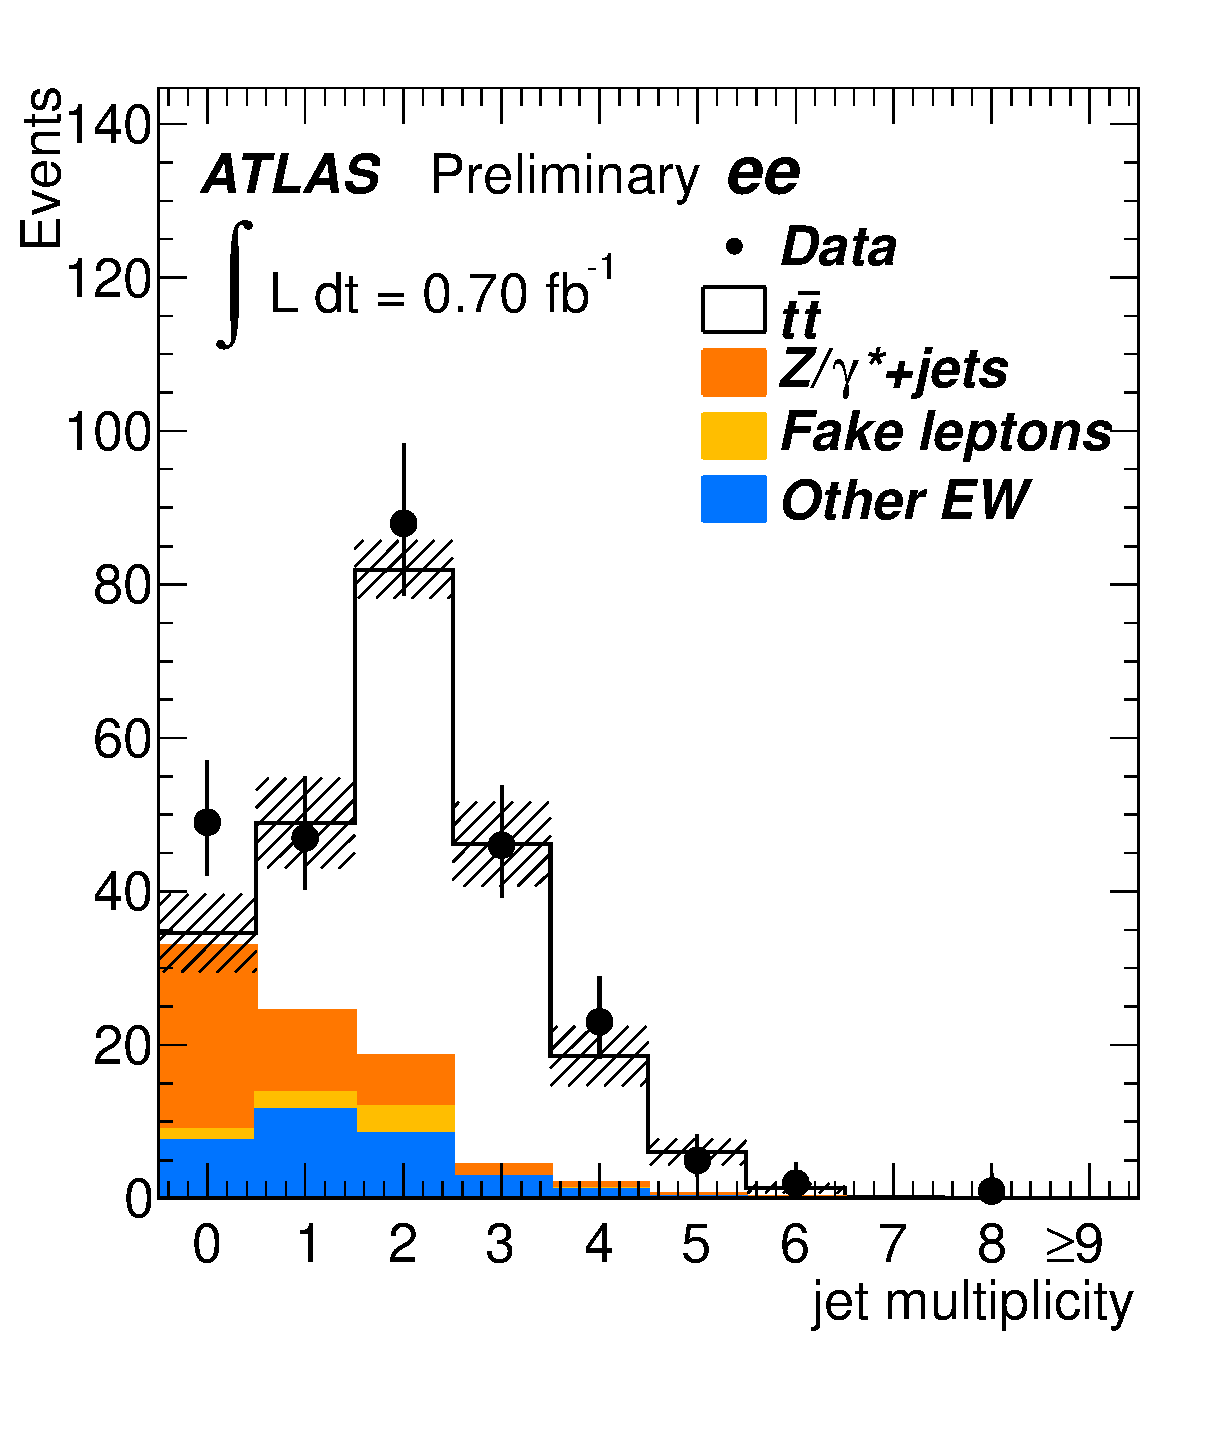
\includegraphics[width=.40\textwidth]{figures/dilep/ee_n_jets} }
    \subfigure[$\mu \mu$]{  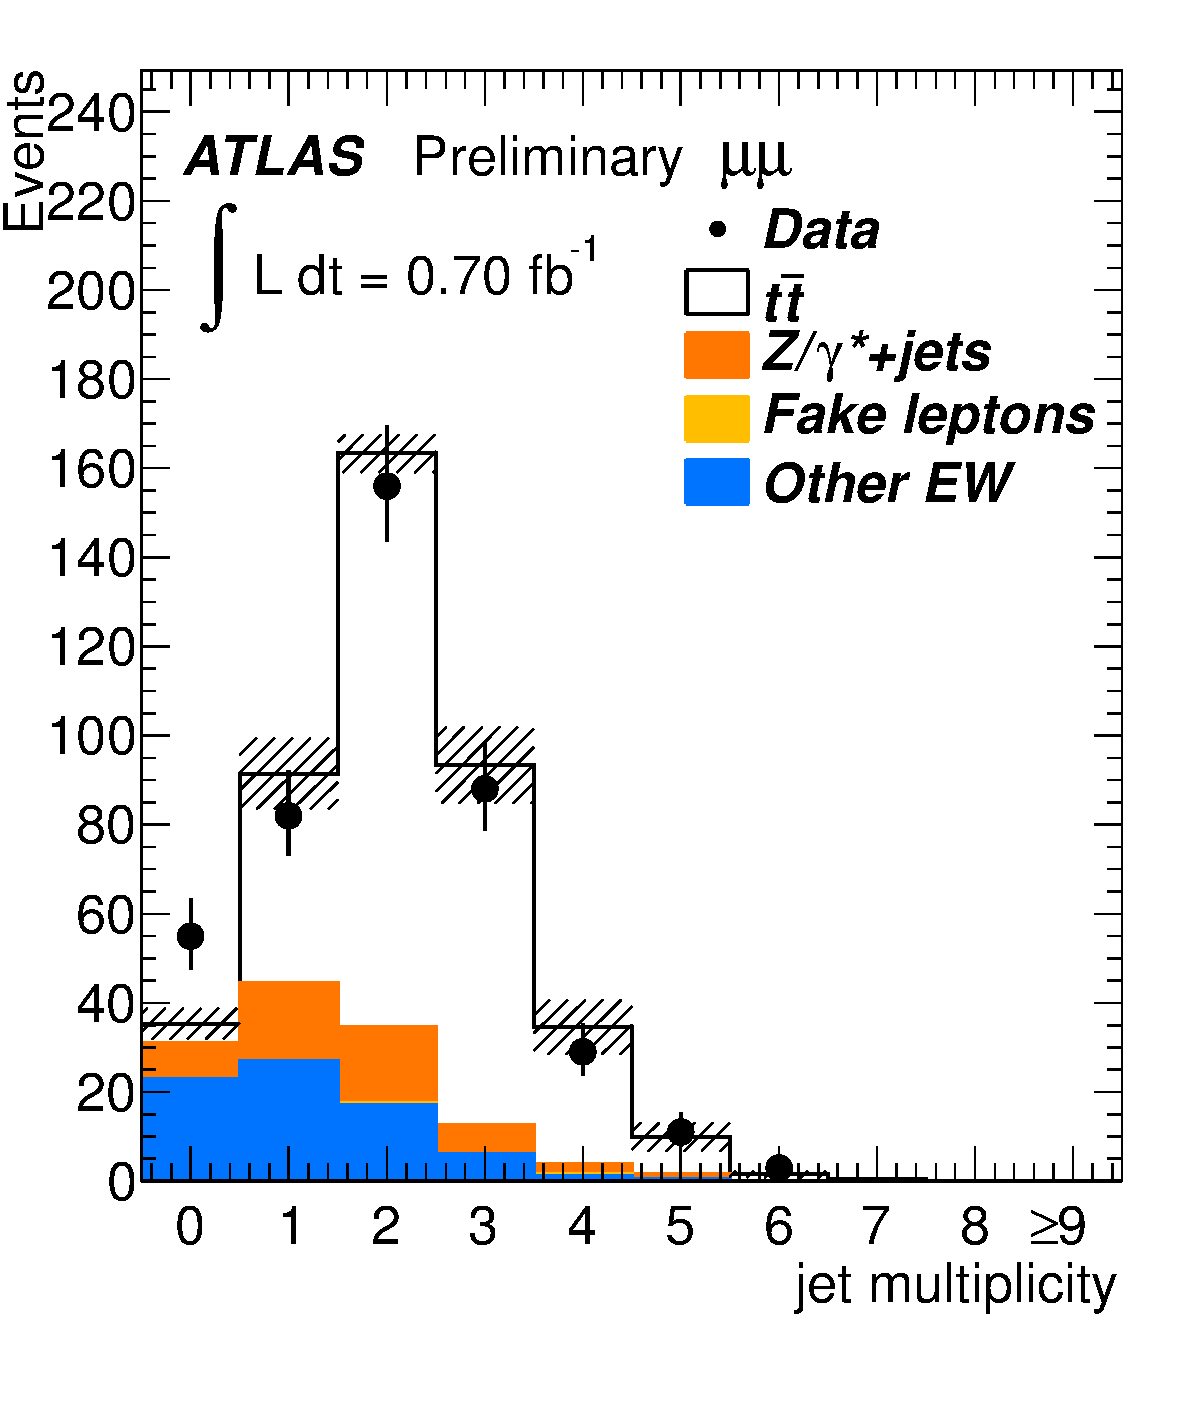
\includegraphics[width=.40\textwidth]{figures/dilep/mm_n_jets} }
    \subfigure[$e \mu$]{    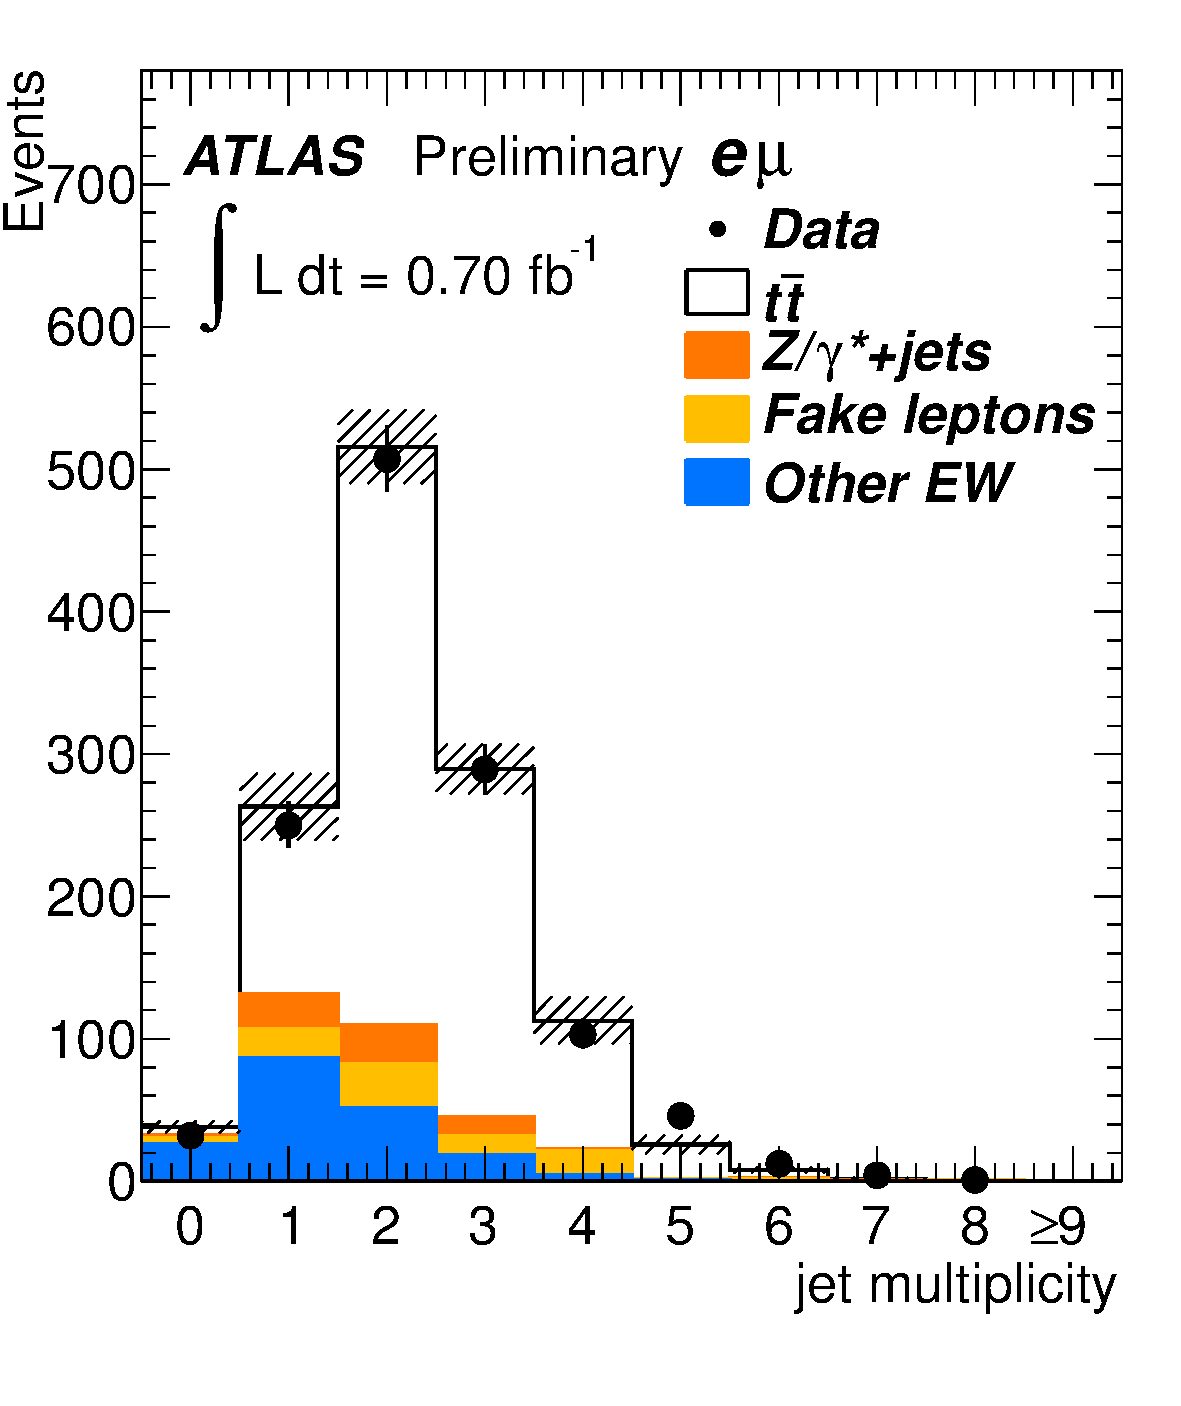
\includegraphics[width=.40\textwidth]{figures/dilep/em_n_jets} }
    \caption{ Jet multiplicity distribution for $ee$, $\mu\mu$, and $e\mu$ events.
      Contributions from diboson and single top-quark events are summarized as `Other EW'.
      Uncertainties shown are statistical and systematic combined.
      The distributions are shown as stacked histograms.}
    \label{f:ll_njets}
  \end{center}
\end{figure}

\begin{figure}[htbp]
  \begin{center}
    \subfigure[$ee$]{       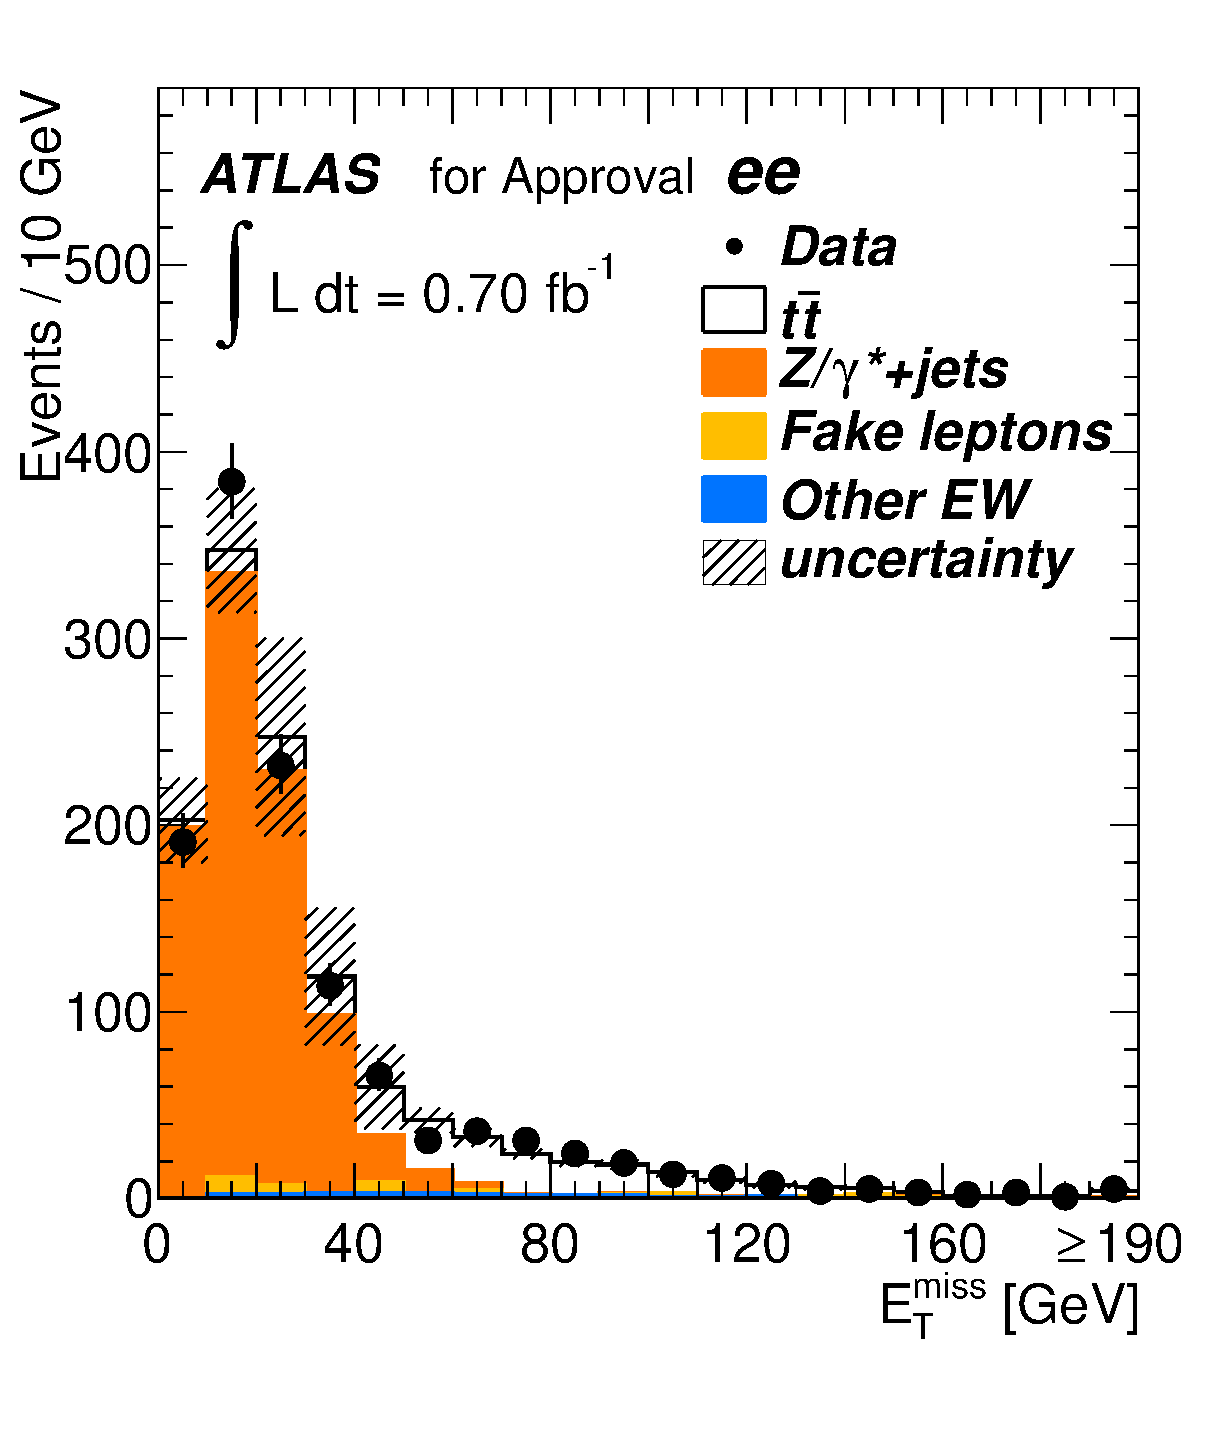
\includegraphics[width=.40\textwidth]{figures/dilep/ee_met} }
    \subfigure[$\mu \mu$]{  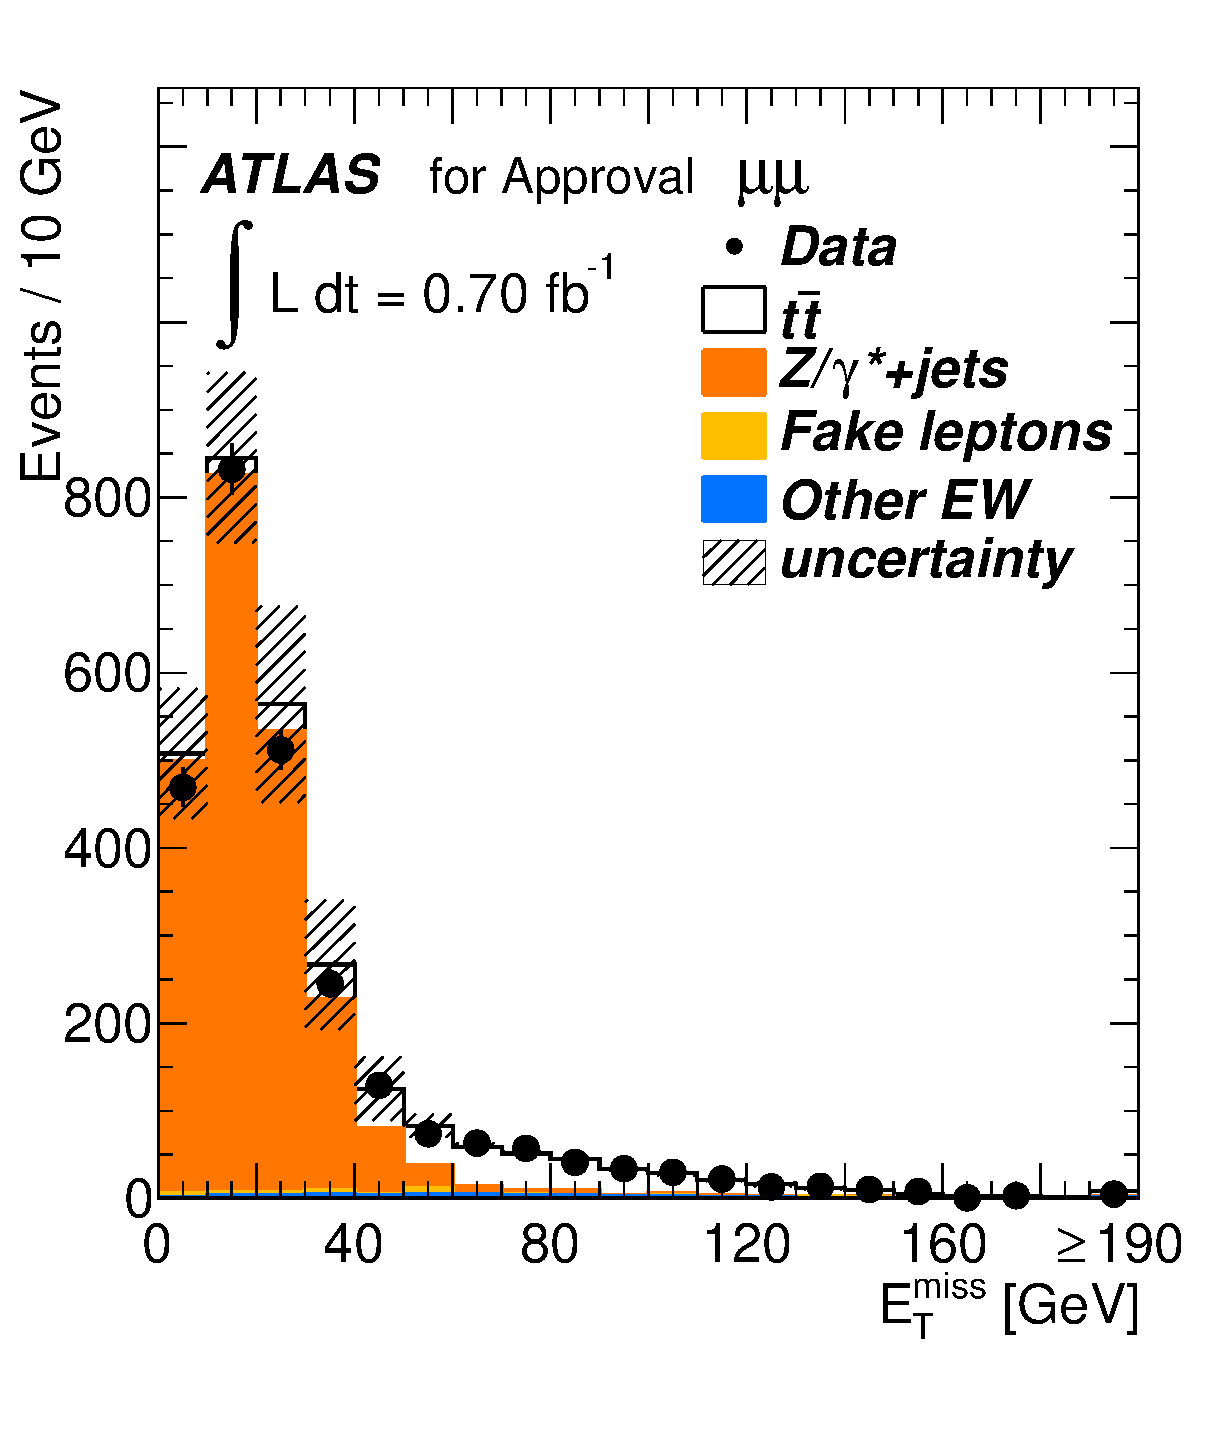
\includegraphics[width=.40\textwidth]{figures/dilep/mm_met} }
    \subfigure[$e \mu$]{    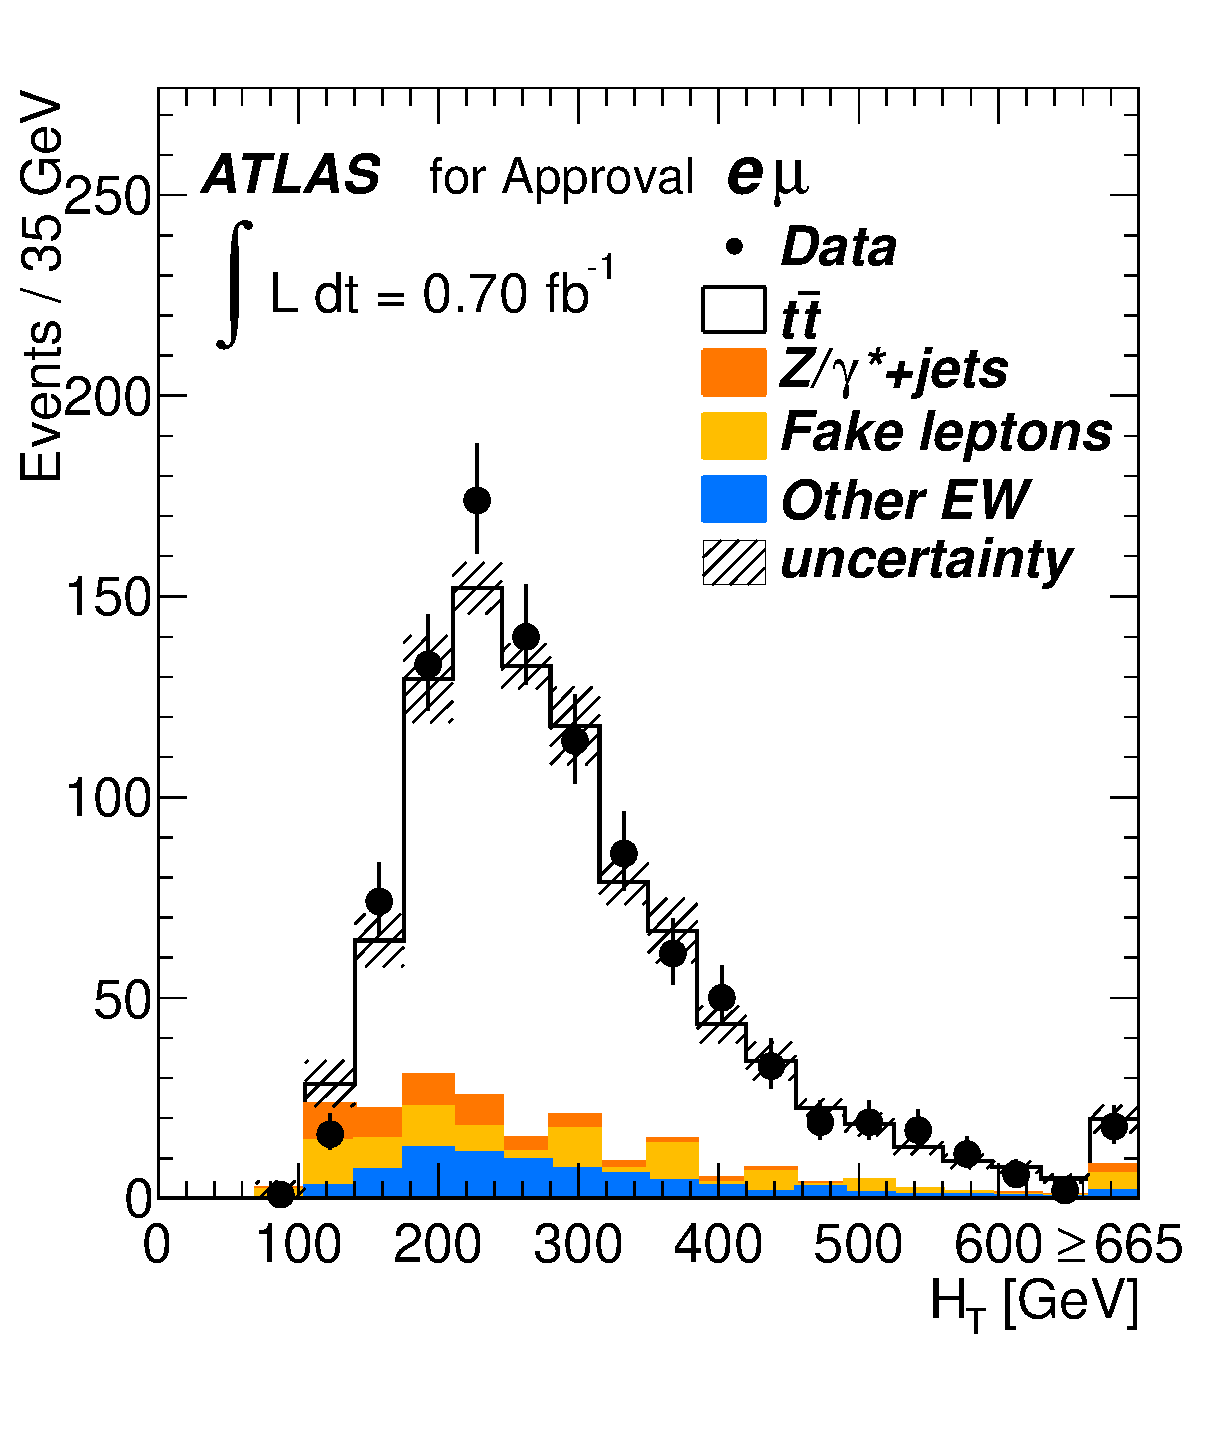
\includegraphics[width=.40\textwidth]{figures/dilep/em_ht} }
    \caption{ Jet multiplicity distribution for $ee$, $\mu\mu$, and $e\mu$ events.
      Contributions from diboson and single top-quark events are summarized as `Other EW'.
      Uncertainties shown are statistical and systematic combined.
      The distributions are shown as stacked histograms.}
    \label{f:ll_met_ht}
  \end{center}
\end{figure}

%% \begin{figure*}
%%   \centering
%%   \subfigure[]{
%%     \includegraphics[width=0.45\textwidth]{figures/dilep/pretag_combined_nJets}
%%   }
%%   \subfigure[]{
%%     \includegraphics[width=0.45\textwidth]{figures/dilep/btag_preTagFinalJetnJetJetProbTaggedJet_all_ATLAS2}
%%   }
%%   \caption{ (a) Jet multiplicity distribution for
%%     $ee$+$\mu\mu$+$e\mu$+$e$TL+$\mu$TL events without a $b$-tagging requirement. (b)
%%     Multiplicity distribution of $b$-tagged jets in the $ee$+$\mu\mu$+$e\mu$ channels. Contributions from diboson and
%%     single top-quark events are summarized as `Other EW'. The
%%     events in (b) are not a simple subset of those in (a) because the
%%     event selections for the $b$-tag and non-$b$-tag analyses differ.
%%     Uncertainties shown are statistical and systematic combined. The
%%     distributions are shown as stacked histograms.}
%%   \label{f:ll_njets}
%% \end{figure*}

%% \begin{figure*}
%%   \centering
%%   \subfigure[]{
%%     \includegraphics[width=0.41\textwidth]{figures/dilep/pretag_combined_Met_log}
%%   }
%%   \subfigure[]{
%%     \includegraphics[width=0.41\textwidth]{figures/dilep/btag_jetProbTaggedInSRMEt_all_logscale_ATLAS2}
%%   }
%%   \caption{
%%     The $\met$ distribution in the signal region for (a) the five
%%     non-$b$-tag channels combined and, (b) the three $b$-tagged channels
%%     combined.  Contributions from diboson and single top-quark events
%%     are summarized as `Other EW'. Uncertainties shown are statistical
%%     and systematic combined. The last bin in each figure is an
%%     overflow bin, including all events above 190 GeV. The distributions
%%     are shown as stacked histograms.}
%%   \label{f:ll_met_ht}
%% \end{figure*}

%The branching fraction for $t\rightarrow Wb$ is taken to be 100\% and the acceptance is calculated for a top mass of 172.5 GeV.
The estimated value of the cross-section is obtained as the maximum
likelihood estimator using the likelihood function produced by
HistFactory, and the uncertainty on that estimation is obtained using
the profile likelihood technique, as described in Ref.~\cite{ATL-CONF-2011-034}. 
The results of this analysis are summarized in table~\ref{tab:dilep_results}.



% Note, the dilepton numbers differ from those in the
% dilepton paper due to the use of separated jes.
\begin{table}[htdp]
  \begin{center}
    \begin{tabular}{|l|c|}\hline
      Channel & $\sigma_{\ttbar}$ (pb) \\ 
      \hline
      & \\
      $ee$      & $186 \pm 17  \textrm{(stat.)} \sp {}^{+31}_{-26} \textrm{(syst.)} \sp {}^{+9}_{-7} \textrm{(lumi.)}$ \\ 
      & \\
      $\mu\mu$  & $167 \pm 12 \textrm{(stat.)}  \sp {}^{+15}_{-11} \textrm{(syst.)} \sp {}^{+8}_{-7} \textrm{(lumi.)}$ \\ 
      & \\
      $e\mu$    & $177 \pm 7  \textrm{(stat.)}  \sp {}^{+15}_{-12} \textrm{(syst.)} \sp \pm 8        \textrm{(lumi.)}$ \\ 
      & \\
      % \hline
      % & \\
      Combined & $173 \pm 6  \textrm{(stat.)}  \sp {}^{+14}_{-11} \textrm{(syst.)} \sp {}^{+8}_{-7} \textrm{(lumi.)}$ \\
      \hline
    \end{tabular}
  \end{center}
  \caption{\label{tab:dilep_results}
    Measured values of $\sigma_{\ttbar}$ obtained in the individual dilepton channels ($ee$, $e \mu$ and $\mu \mu$) and well as the three-channel dilepton combination.}
\end{table}

